\documentclass{article}
\usepackage{color}
\usepackage{graphicx}
\usepackage{amsmath,amssymb,amsthm}
\usepackage[margin=0.75in]{geometry}

\newcommand{\ind}{\mathbb{I}} % Indicator function
\newcommand{\pr}{\mathbb{P}} % Generic probability
\newcommand{\ex}{\mathbb{E}} % Generic expectation
\newcommand{\normal}{\mathcal{N}} % Generic expectation
\newcommand{\var}{\textrm{Var}}
\newcommand{\cov}{\textrm{Cov}}
\newcommand\independent{\protect\mathpalette{\protect\independenT}{\perp}}
\def\independenT#1#2{\mathrel{\rlap{$#1#2$}\mkern2mu{#1#2}}}
\theoremstyle{plain}
\newtheorem{theorem}{Theorem}

\setlength{\parindent}{0cm}


\title{Simulation}
%\date{}               

\begin{document}
\maketitle


\section{Simulation Design}
RCT eligibility, complier status, and treatment assignment in the population depend on observed covariates. 
The observed covariates $(W_1, W_2, W_3)$ are multivariate normal with mean $(0.5, 1, -1)$ and covariances $\cov(W_1, W_2) = 1$ and $\cov(W_1, W_3) = \cov(W_2, W_3) = 0.5$. 
 The  equation for selection into studies is
 $$ S = \ind(e_2 + g_1W_1 + g_2W_2 + g_3W_3 + R > 0)$$
  where $R$ is standard normal. $e_2$ controls the fraction of the population eligible for the RCT. We set $g_1, g_2,$ and $g_3$ to be $0.5, 0.25,$ and $0.75$, respectively.
The compliance indicator is determined by
$$C = \ind(e_3 + h_2W_2 + h_3W_3 + Q > 0)$$
where $Q$ is standard normal. $e_3$ controls the fraction of compliers in the population. We set $h_2$ and $h_3$ to $0.5$.
 In the population (individuals with $S=0$),  treatment is assigned by
  $$T = \ind(e_1 + f_1W_1 + f_2W_2 + V > 0)$$
Varying $e_1$ controls the fraction eligible for treatment in the population. $V$ is standard normal. We set $f_1$ to $0.25$ and $f_2$ to $0.75$.  For individuals in the RCT ($S=1$), treatment assignment is a sample from a Bernoulli distribution.
We set treatment received $D$ according to $T$ and $C$: $D = T$ if $C=1$ and $D = 0$ if $C=0$.
Finally, the response $Y$ is determined by 
$$Y = a + bD + c_1W_1 + c_2W_2 + dU$$
 We assume that the treatment effect $b$ is heterogeneous depending on $W_1$: $b = 1$ if $W_1 > 0.75$ and $b=-1$ if $W_1 \leq 0.75$.   We set $a, c_1,$ and $d$ to $1$ and $c_2$ to $2$. $U$ is standard normal and $U, V, R, Q, (W_1, W_2, W_3)$ are mutually independent.\\
 
 We generate a population of 30,000 individuals and randomly sample 5,000.  Those among the 5,000 who are eligible for the RCT ($S=1$) are selected. Similarly, we sample 5,000 individuals from the population and select those who are not eligible for the RCT ($S=0$); these are a sample of the ``target population''.  We set each individual's treatment received $D$ according to their treatment assignment and complier status and observe their responses $Y$.  In the assigned-treatment RCT group $(S = 1, T = 1)$, we fit a logistic regression to compliance status using the covariates.  With this model, we predict who in the control group $(S = 1, T = 0)$ has $C=1$, since this is unobservable.  These individuals \textit{would have} complied had they been assigned to the treatment group.  We do the same for the target population control group.  \\
 
For this group of observed compliers to treatment and predicted compliers from the control group of the RCT, we estimate the response curve using a random forest with features $(W_1, W_2, W_3)$ and $D$.  Then population local average treatment effect on the treated is estimated according to Theorem 1.


\section{Results}

\begin{figure}[htbp]
\begin{center}
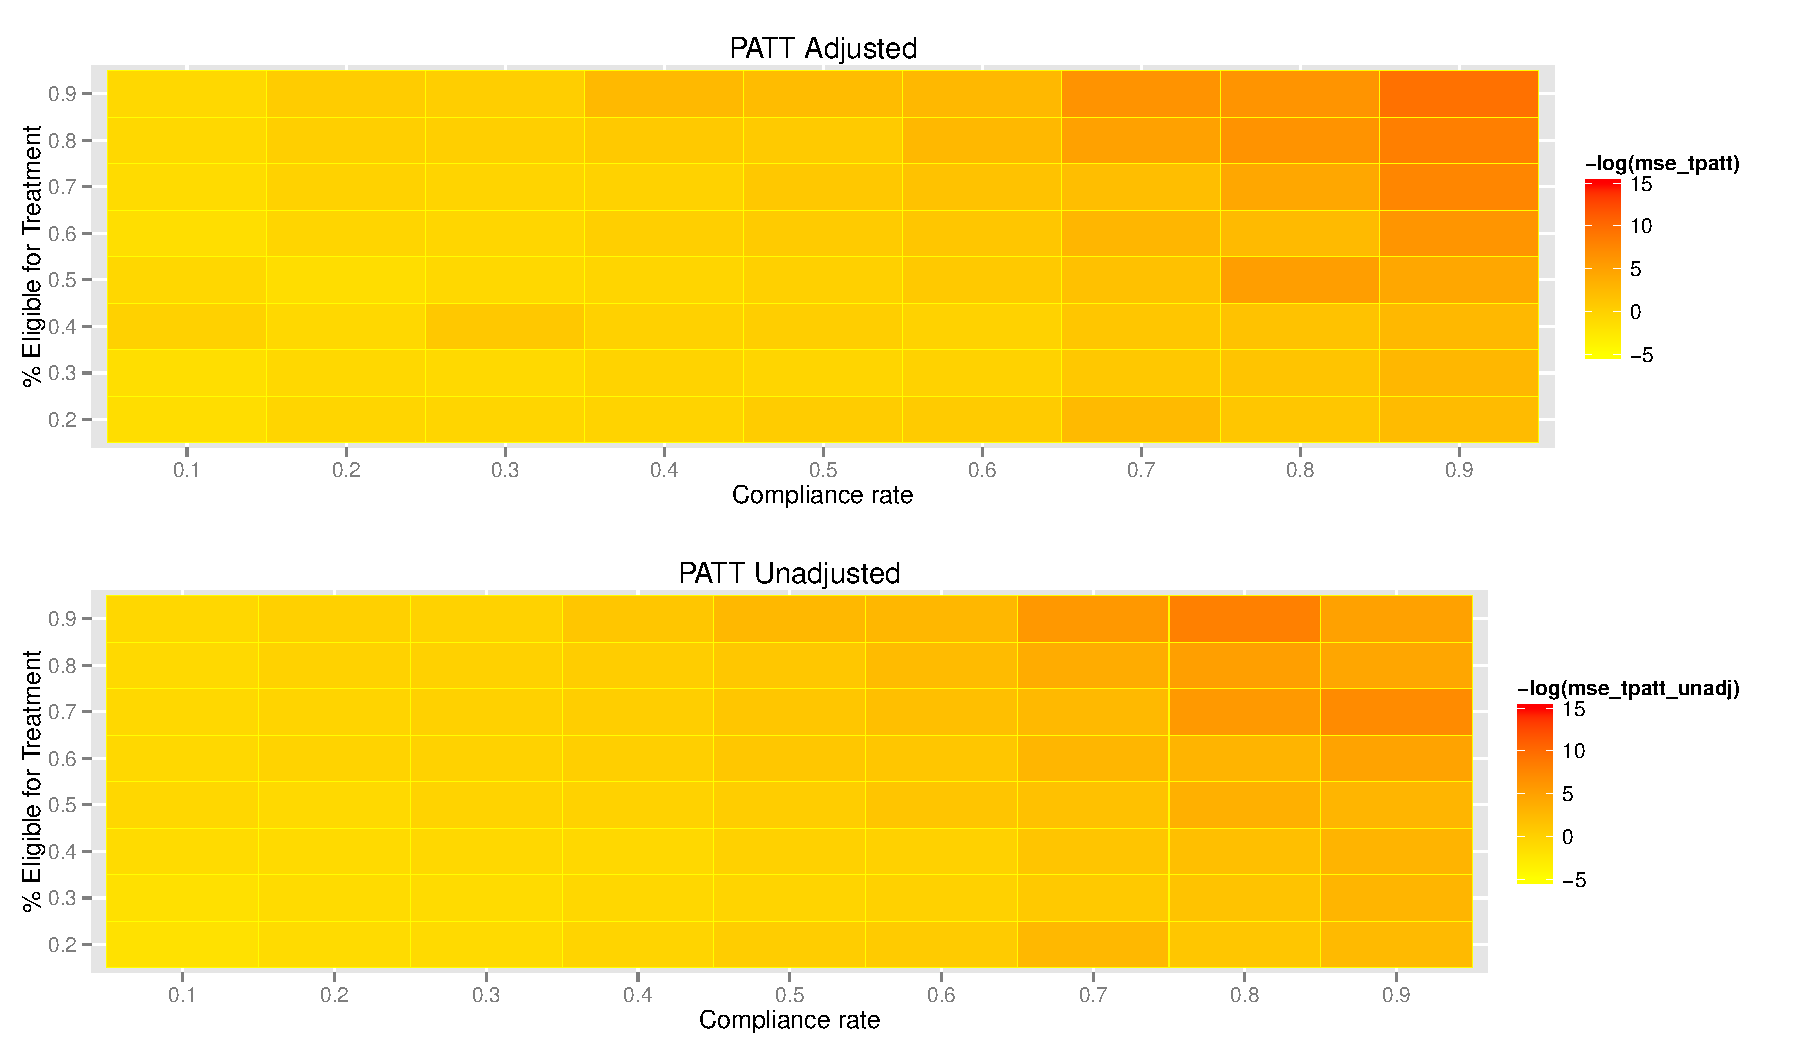
\includegraphics[width = 0.8\textwidth]{mse_ratec_ratet}
\caption{Simulated mean squared error, transformed by $-\log$. Darker tiles correspond to lower mean squared error.}
\label{default}
\end{center}
\end{figure}
\begin{figure}[htbp]
\begin{center}
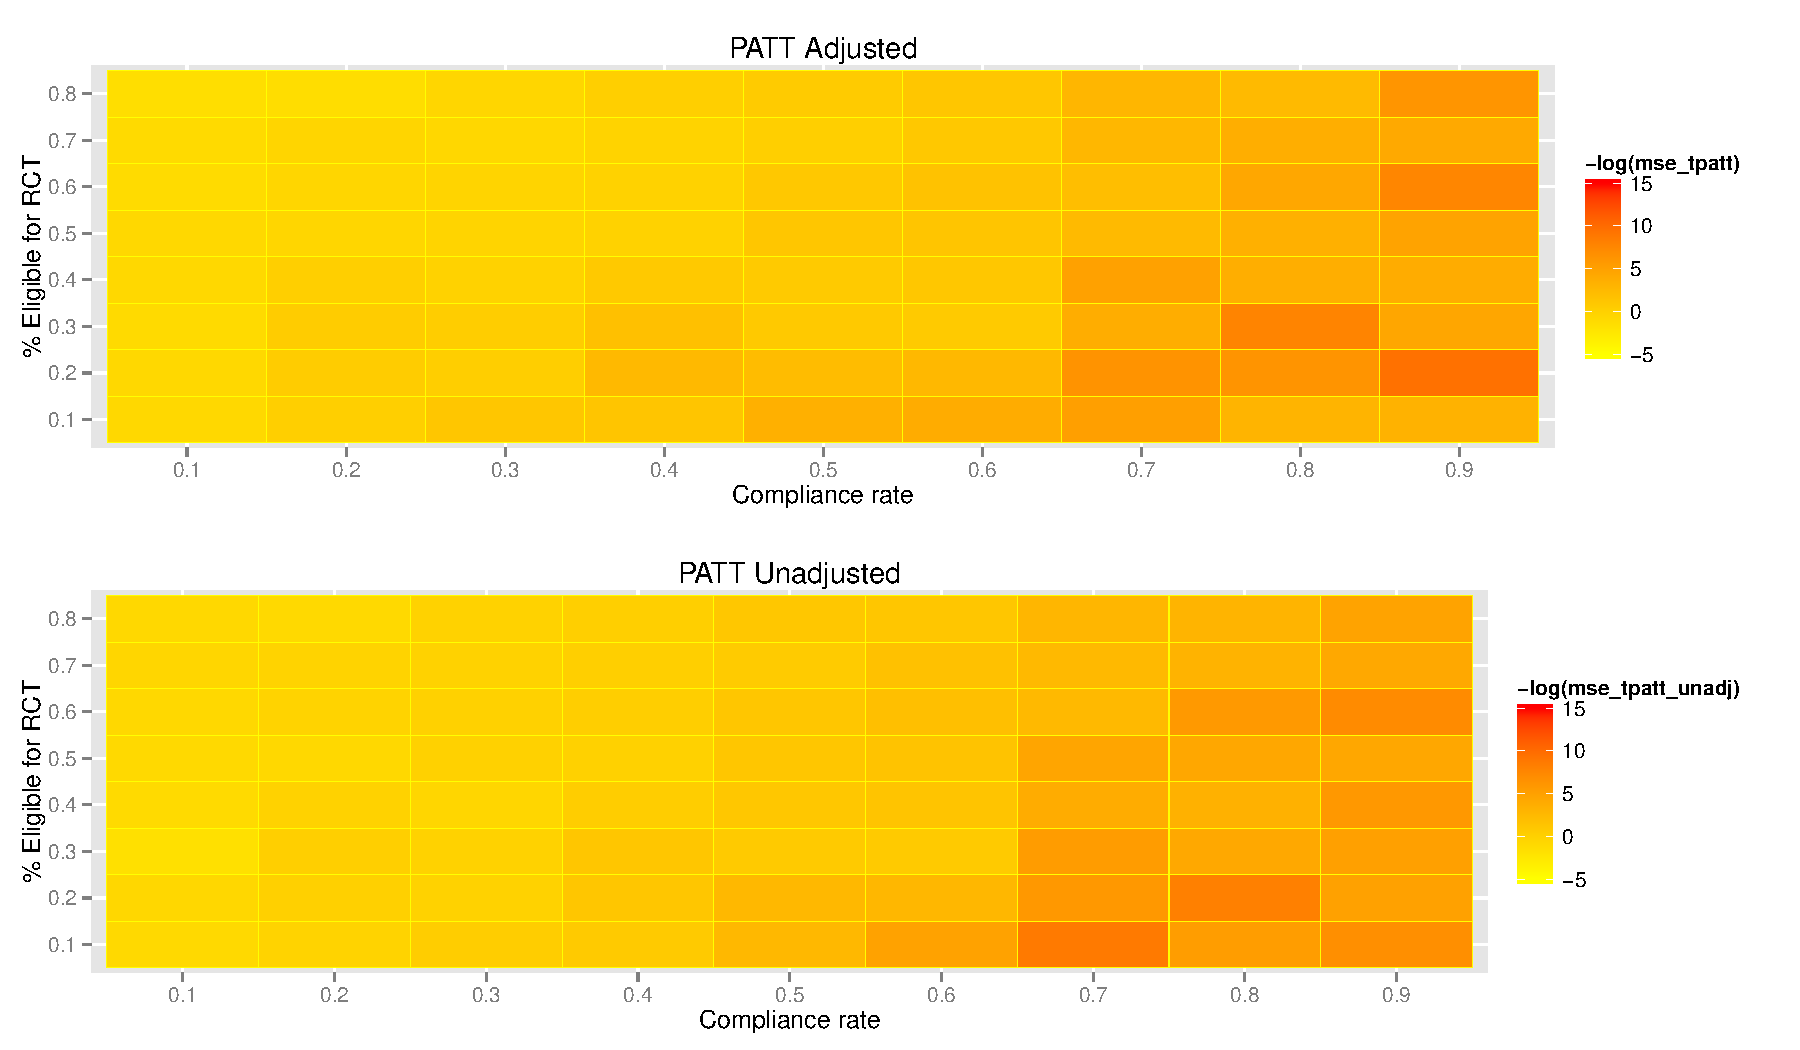
\includegraphics[width = 0.8\textwidth]{mse_ratec_rates}
\caption{default}
\caption{Simulated mean squared error, transformed by $-\log$. Darker tiles correspond to lower mean squared error.}
\end{center}
\end{figure}
\end{document}  